% id: 47-11
% book: 베이직쎈 확률과 통계 · 03 확률의 뜻과 활용
% section: 유형 026 중복순열을 이용하는 확률
% figure: crop:fig-47-11.jpg
% answer: 
% answer_source: 
% variant_level: 0 (원본 전사)
% 이 파일은 build.mjs 가 items.json 에서 만든다. 고칠 때는 items.json 을 고친다.
\smash{\raisebox{1.5mm}{\dmkichul{베이직쎈 확률과 통계 47쪽 11번}}}
\noindent\begin{minipage}[t]{0.58\linewidth}\vspace{0pt}\raggedright 어느 분식집에서는 야채김밥, 참치김밥, 치즈김밥, 김치김밥만을 판매하고 있다. 이 분식집에서 민주와 재희가 각각 김밥을 한 줄씩 구매할 때, 두 사람이 같은 종류의 김밥을 구매할 확률을 구하시오.\end{minipage}\hfill\begin{minipage}[t]{0.4\linewidth}\vspace{0pt}\centering 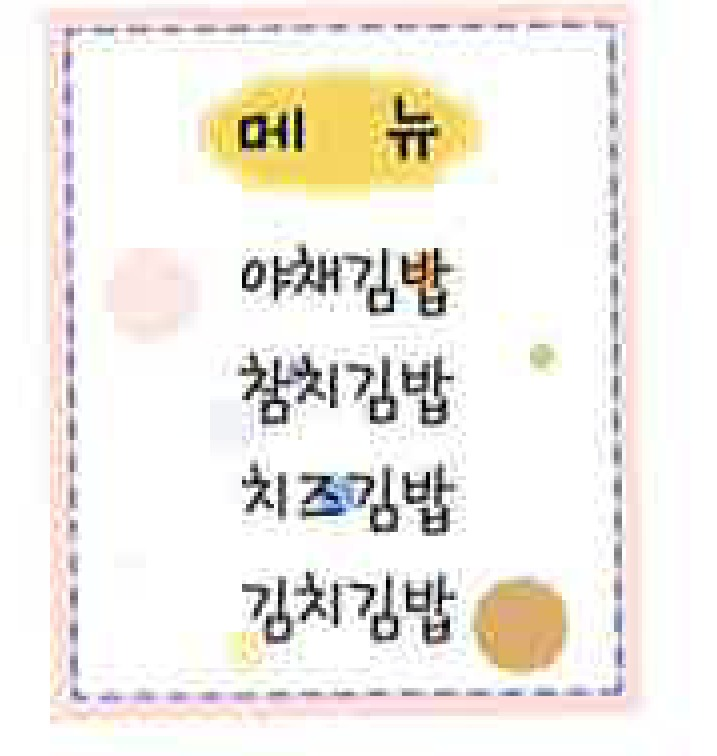
\includegraphics[width=0.92\linewidth]{figures/fig-47-11.jpg}\end{minipage}\par
